\documentclass[12pt, french]{article}
\usepackage{fontspec}
\setmainfont{Arial}
\usepackage{wrapfig}
\usepackage[french]{babel}

\usepackage{setspace}
\singlespacing

%\usepackage[none]{hyphenat}

\usepackage{graphicx}
\usepackage{caption}
%\usepackage[T1]{fontenc}
%\usepackage[utf8]{inputenc}
\usepackage{lmodern}
\usepackage{geometry}
\geometry{
	a4paper,
	left=20mm,
	right=20mm,
	top=25mm,
	bottom=25mm,
}

\usepackage{pgfgantt}
\usepackage{eurosym}

\usepackage{pdfpages}


\usepackage{subcaption}

\usepackage[unicode=true,pdfusetitle,bookmarks=true,bookmarksnumbered=false,bookmarksopen=false,
breaklinks=false,pdfborder={0 0 0},backref=false,colorlinks=true,urlcolor=magenta]{hyperref}

\usepackage{multibib}
\newcites{article,conf,confnoproc}{{Articles dans des revues internationales à comité de lecture
	},{Communications dans des congrès internationaux à comité de lecture et actes
		publiés},{Communications dans des congrès internationaux sans comité de lecture}}


\newcommand{\review}[1]{\textcolor{blue}{#1}}

\graphicspath{{images/}}

\author{Andrea Brugnoli \\ 
	\hspace{2.8pt} Docteur ISAE-SUPAERO 2020\\
	Ingénieur ISAE-SUPAERO 2017}
\title{Project MORPHEUS \\
	\vspace{.3cm}
	\Large{Model Order Reduction for multi-PHysical and Energy-Unified Systems}  }

\date{}

\begin{document}
	
	\maketitle
	
	\large{\noindent Candidat sélectionné par ISAE-SUPAERO pour candidater au prix de la fondation Jean-Jacques et Félicia Lopez-Loreta pour l'excellence académique. }

	
	
	\begin{figure}[h]
		\centering
		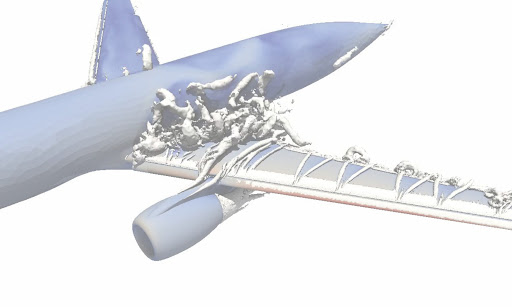
\includegraphics[width=.95\textwidth]{3Dplane.jpg}
		\captionsetup{labelformat=empty}
		\caption{Source: \href{http://www.fenics-hpc.org/}{FEniCS-HPC website}}
	\end{figure}
	
	
	
	
	
	\thispagestyle{empty}
	
	\newpage
	
	\tableofcontents
	\newpage
	
	
	\section{Résumé du projet}
	
	Le but du projet MORPHEUS consiste à mettre en place des méthodes numériques
	pour accélérer la simulation des problèmes d'interaction fluide-structure (IFS), par rapport au temps de calcul requis pour une simulation haute-fidélité. Il sera donc possible d'intégrer des modèles plus économiques, qui pourront remplacer des simulations très coûteuses. Cela permettra également de faciliter le design optimisé des composantes du système et la prise de décision. À la différence de plusieurs méthodes proposées dans la littérature, l'impératif est la fidélité à la structure physique du problème.  Cette structure est le plus souvent ignorée par les algorithmes de réduction, qui traitent les simulations comme des boîtes noires. Les modèles réduits respectueux de la physique sont beaucoup plus précis que ceux qui ne la garantissent pas et leur utilisation pourra radicalement améliorer les techniques normalement utilisées pour l'optimisation. Pour réaliser son ambition, ce projet vise à utiliser des formalismes mathématiques récents pour la modélisation multiphysique et la digitalisation des modèles. Les outils capables de prédire le comportement des systèmes complexes ont une importance fondamentale pour nous aider à affronter les prochains défis technologiques et sociétaux. Le fait que cette année le Prix Nobel de Physique ait été attribué à trois chercheurs travaillant sur ce sujet\footnote{\url{https://www.nobelprize.org/prizes/physics/2021/summary/}} confirme
	l'importance et l'actualité de cet axe de recherche.
	
	
	\section{Développement du projet scientifique}
	
	\subsection{Les problèmes multiphysiques}
	L'ingénierie computationnelle est une science récente, multidisciplinaire et en expansion rapide. Son but consiste à mettre en place des modèles mathématiques et numériques pour prédire le comportement des systèmes complexes. Cela permet de concevoir des systèmes ex novo ou bien de détecter des fautes pendant le cycle de vie des composants, sans devoir utiliser des tests expérimentaux très co\^{u}teux. Ce domaine est en expansion rapide car aujourd'hui on dispose d'ordinateurs plus puissants et surtout parce que les algorithmes ont été optimisés pour être plus rapides, robustes et faciles à utiliser. Toutefois les problèmes multiphysiques, qui sont centraux dans les applications industrielles, sont extrêmement compliqués à traiter. Cela est d\^u d'une part à la difficulté associée au traitement des différentes physiques et d'autre part à la taille des systèmes obtenus, qui nécessitent plusieurs jours, voire plusieurs semaines, pour être résolus à l'aide d'un supercalculateur \cite{keyes2013}. Ces problématiques posent des barrières pour l'utilisation des modèles numériques en industrie. 
	
	
	\subsection{Outils scientifiques du projet MORPHEUS}
	
	
	\paragraph{\large Un formalisme unificateur pour la modélisation des systèmes dynamiques\\}
	Un formalisme mathématique très prometteur pour traiter les problèmes multiphysiques est le formalisme port-Hamiltonien \cite{vanderSchaft2002}, basé sur la mécanique Hamiltonienne et les graphes de liaisons pour la modélisation des systèmes dynamiques (cf. l'annexe \ref{sec:pHreview} pour plus de détails sur cette théorie). Au c\oe{}ur de ce formalisme, il y a l'idée que tout système physique peut être décrit d'une manière modulaire. C'est-à-dire à partir des ses composantes simples, interagissant entre eux et avec le milieu environnant à travers des portes. Les portes d'interaction contiennent l'information relative au flux d'énergie entre les différents composants et entre différents domaines physiques: mécanique, électromagnétisme ou dynamique des fluides. La conception modulaire est centrale dans l'ingénierie, car le design de tout système technologique est fait à partir des éléments simples qui sont assemblés pour donner lieu à la complexité qui nous entoure. Prenez par exemple un avion, un hélicoptère, un satellite (cf. Fig. \ref{fig:satellite}) : pour pouvoir optimiser leur design il est indispensable de disposer d'un outil de modélisation capable de décomposer la complexité de manière à retrouver les différents composants clés. Le fait d'utiliser un outil de modélisation unifié représente une nouveauté essentielle de ce projet. Cela pourra permettre la création d'une infrastructure commune pour les outils numériques à la base de la digitalisation, afin de faciliter son adoption dans l'industrie.
	
	\begin{figure}[hb]
		\centering
		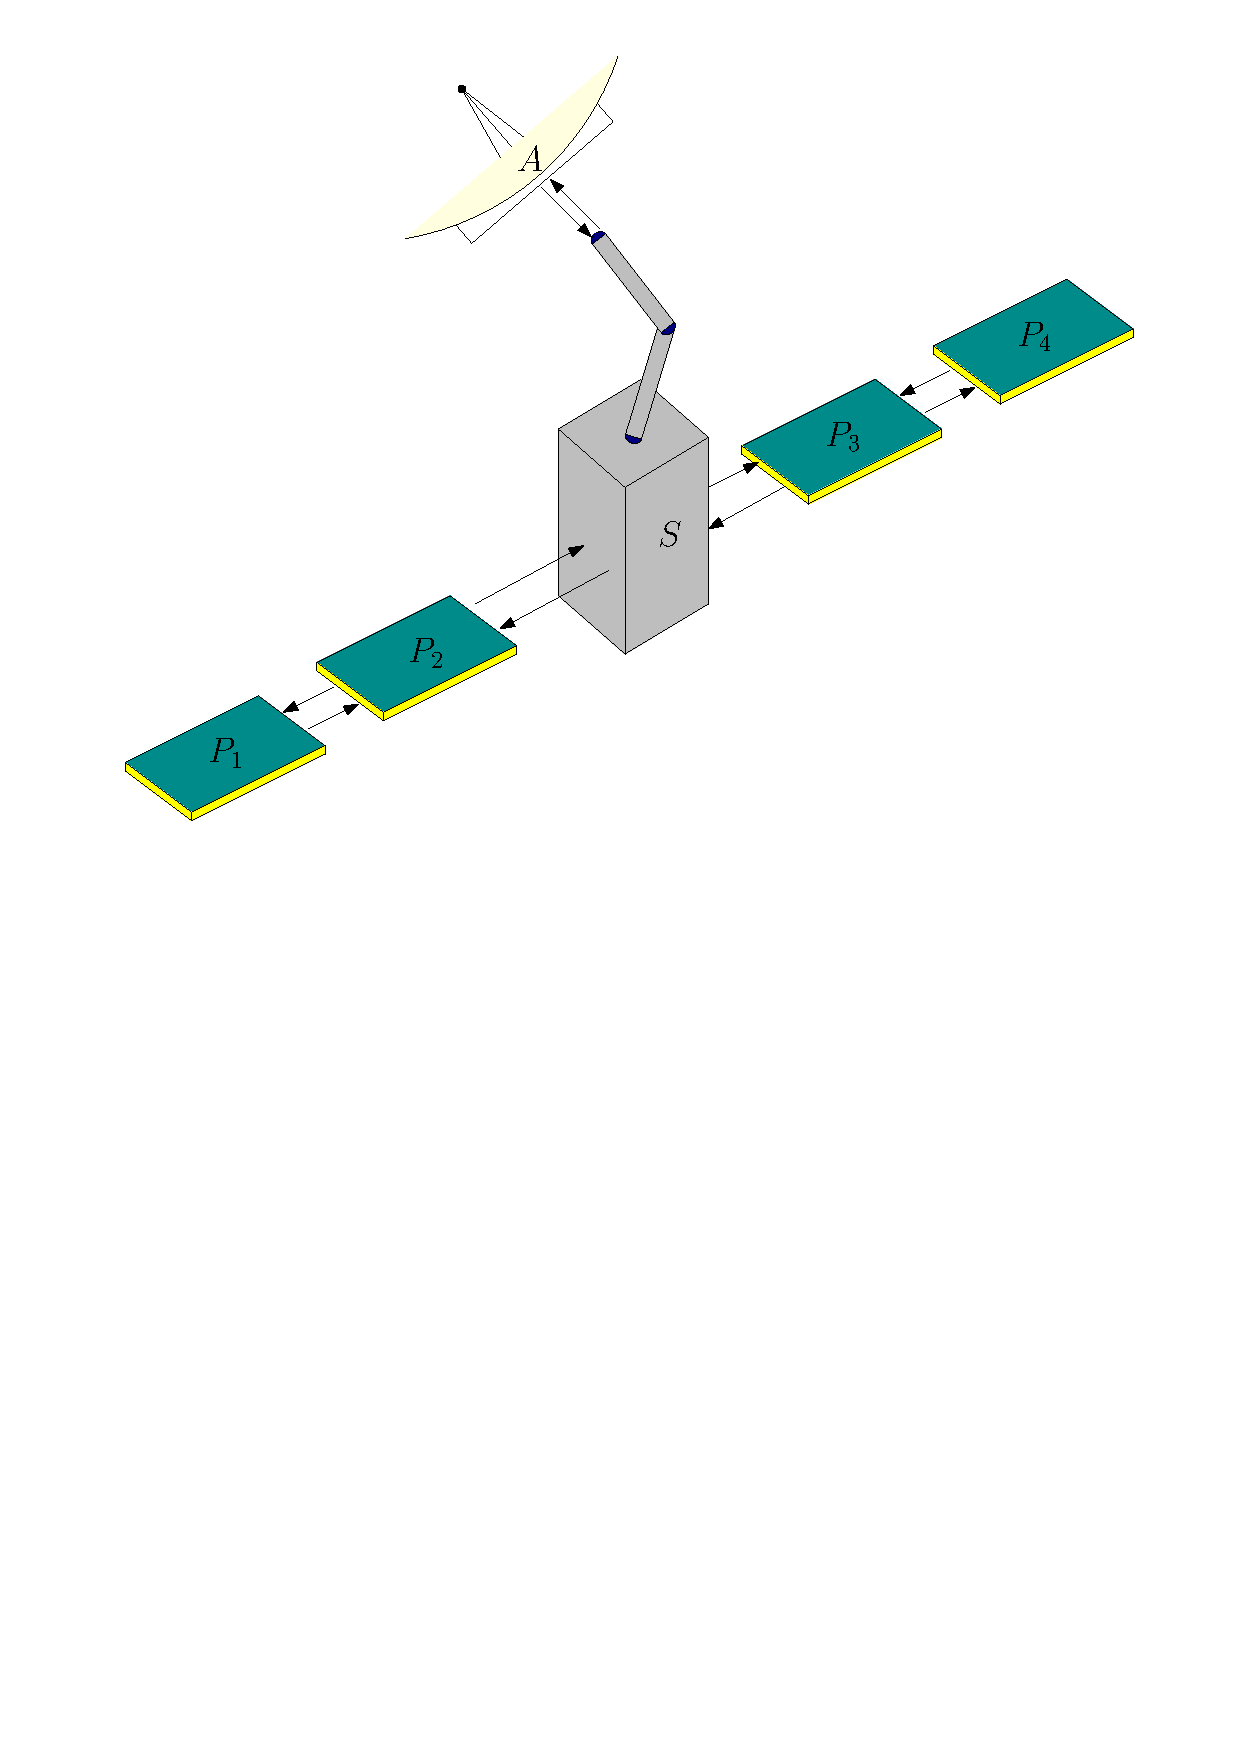
\includegraphics[width=.6\textwidth]{satellite.pdf}
		\caption{Schéma modulaire représentant un satellite de télécommunication.}
		\label{fig:satellite}
	\end{figure}

	\paragraph{\large Une méthodologie structurée pour la discrétisation \\}
	Les algorithmes numériques utilisés en industrie sont adaptés à la nature physique du problème. Pour la mécanique des solides, la méthode des éléments finis est privilégiée par les ingénieurs. Pour la dynamique des fluides, les volumes finis sont majoritairement utilisés car il garantissent le respect des lois de conservation. Quand il faut utiliser ces deux approches simultanément, leur couplage pose plusieurs défis. Les deux méthodes utilisent des degrés de liberté différents (i.e. différentes entités topologiques du maillage) et l'interconnexion introduit forcément des erreurs. Un outil de modélisation général nécessite une méthode de discrétisation également générale, capable de  garantir la possibilité d'interconnecter des physiques distinctes. Récemment, un formalisme unificateur pour la discrétisation des équations à dérivées partielles  à été développé  \cite{arnold2006acta}. Cette théorie mathématique, appelée la méthode des éléments finis en calcul extérieur or FEEC\footnote{Le calcul extérieur représente une généralisation du calcul vectoriel basée sur la géométrie différentielle.}, a permis des développements importants pour la discrétisation des équation aux dérivées partielles issues de la physique. Elle à été appliquée avec succès au cas de la mécanique des solides, la dynamique des fluides et l'électromagnétisme et elle représente un outil puissant pour les applications multiphysiques. La portée de cette théorie est illustrée par le fait que le Royaume-Uni a décidé d'utiliser cette nouvelle méthode pour renouveler les codes de calcul pour la météorologie\footnote{Le site \url{https://www.metoffice.gov.uk/research/news/2021/gungho-and-lfric-10th-anniversary} donne un aperçu du projet. Le lecteur intéressé peut aussi consulter les planches  \url{https://www.ecmwf.int/sites/default/files/elibrary/2016/16815-introduction-lfric-project.pdf}}.
	
	\paragraph{\large L'intelligence artificielle pour obtenir des modèles réduits\\}
	Toute méthode de discrétisation, même la plus sophistiquée, amène à des systèmes dont la taille dépasse facilement le million d'inconnues. Pour pouvoir optimiser le design des composantes mécaniques, il faut simuler ces modèles plusieurs fois. Cela amène à des coûts computationnels prohibitifs même pour les entreprises dotés des centres de calcul les plus avancés. Il est donc indispensable d'introduire des méthodes de réduction, qui sont censées construire un modèle plus simple, capable néanmoins de retenir les propriétés principales du système de départ. La grande majorité de ces méthodes suppose que l'on puisse obtenir un système réduit à travers une méthode essentiellement linéaire, i.e. la Décomposition Orthogonale en Valeurs Propres (POD) \cite{shinde2019,tello2020fluid}. Cette hypothèse n'est pas valable pour tout système exhibant un comportement non-linéaire et conduit à surestimer la dimension du système réduit. Grâce aux progrès récents dans le domaine de l'Intelligence Artificielle (IA), de nouvelles méthodes permettent d'obtenir des modèles réduits plus performants. Par exemple, des chercheurs ont proposé une architecture basée sur les réseaux neuronaux convolutifs \cite{lee2020} pour obtenir des modèles beaucoup plus rapides (d'un facteur 100 environ) par rapport aux discrétisations haute fidélité. Leur technique représente une extension non linéaire des méthodologies couramment utilisées. Les résultats obtenus démontrent le gain de performances qu'il est possible d'obtenir en utilisant les réseaux neuronaux convolutifs (cf. Fig. \ref{fig:deepROM}).
	
	\begin{figure}[t]
		\begin{subfigure}[t]{0.465\textwidth}
			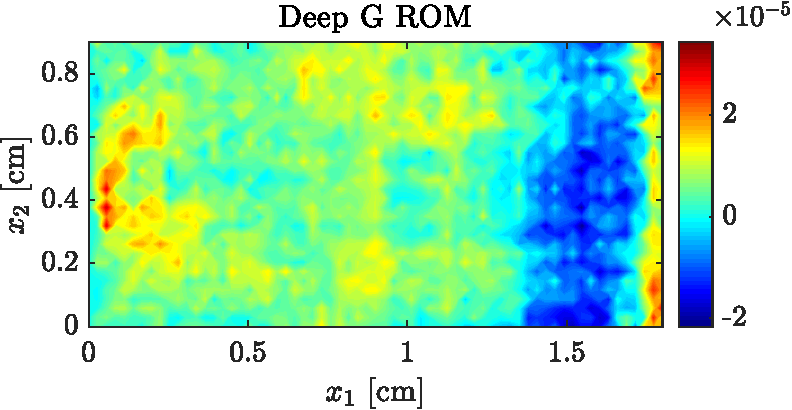
\includegraphics[width=\columnwidth]{DGROM_T_param1.pdf} 
			\caption{Modèle réduit avec réseaux des neurones.}
			\label{fig:DG_ROM}
		\end{subfigure}\hfill
		\begin{subfigure}[t]{0.48\textwidth}
			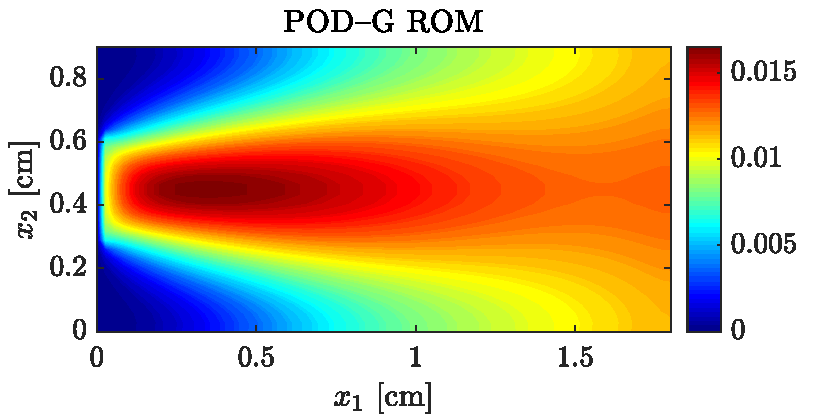
\includegraphics[width=\columnwidth]{GROM_T_param1.pdf}%
			\caption{Modèle réduit avec la méthode linéaire POD.}
			\label{fig:POD_ROM}
		\end{subfigure}
		\caption[]{Erreur des modèles réduits sur le champ de température pour un problème de convection-diffusion-réaction. En utilisant un réseau neuronal convolutifs pour générer une variété non linéaire (cf. Fig. \ref{fig:DG_ROM}) l'erreur associée à la réduction  est drastiquement réduite, de $10^{-2}$ à $10^{-5}$, par rapport à la méthode POD (cf. Fig. \ref{fig:POD_ROM}). Reproduit de \cite{lee2020} avec permission.}%
		\label{fig:deepROM}%
	\end{figure}


\subsection{Verrous scientifiques et lots de travaux pour les adresser}
Le premier défi est liée \`a la résolution des systèmes couplés multiphysiques.  Dans l'industrie des méthodes différentes sont habituellement utilisées pour simuler des physiques distinctes. Par conséquent, le couplage numérique ne représente pas correctement les flux d’énergie. Il est souvent nécessaire d'integrer différents solveurs et logiciels pour pouvoir simuler ces problèmes. Cela amène \'a une complexification des procédures industriels. \\

Le premier lot de travail (\textbf{WP1}) cherche à résoudre les problématiques liées au couplage multiphysique, d'une manière a garantir le respect des fluxes d'energie entre différentes physiques. Ces modèles numériques devront retenir les propriétés physiques du problème (conservation d’énergie globale, traçage des échanges d’énergie entre les différents sous-systèmes, invariants du problème). \\

\begin{itemize}
	\item \textbf{WP1} : Développement d'algorithmes numériques haute-fidélité pour des problèmes d'interactions fluide-structures, basés sur les élément finis en calcul extérieur et le formalisme port-Hamiltonien. \\
\end{itemize}

L’utilisation d’un paradigme de modélisation unifié permettra d’effectuer les couplages de manière à respecter la physique.\\

Le second verrous scientifique du projet consiste à intégrer des techniques issues de l'IA, qui seront utilisées pour obtenir des modèles réduits physiques. Il s'agit d'un thème de recherche récent mais en expansion rapide. Pour le moment, l'intelligence artificielle est utilisée majoritairement pour automatiser des taches simples, comme la classification automatique des images, du texte, des vidéos, etc. Malgré les exploits récents des algorithmes capables de surpasser les hommes dans le jeux de société comme les échecs ou le go, l'utilisation de l'IA pour la physique computationelle est encore dans un état embryonnaire. Il est extrêmement important de comprendre les avantages et limitations de ces techniques pour les intégrer à l'ensemble des outils numériques qui ont déjà fait leurs preuves dans la modélisation physique. \\

Le deuxième lot de travail (\textbf{WP2}) a comme but la génération des modèles réduits capables d'incorporer la physique du problème d'une manière interprétable. \\

\begin{itemize}
	\item \textbf{WP2} : Méthodes de réduction garantissant le respect de la structure physique implémentées en utilisant les réseaux des neurones.\\
\end{itemize}

Ce lot de travail consentira d'obtenir des modèles de petite dimension, prêts à être utilisés pour la partie optimisation.\\ 

L'optimisation et les études paramétriques sont typiquement effectuées sur les
modèles de substitution en industrie, car optimiser directement les modèles fins entraîne des coûts computationels absolument prohibitifs. Il est très difficile de savoir \`a l'avance quel méthode utiliser pour générer un modèle de substitution un certain problème physique \cite{lancaster2018}. La fiabilité des ces modèles est également difficile \'a prévoir, vu que le sens physique du problème est détruit par la procédure de réduction. \\

Le dernier objectif du projet est de démontrer que les modèles réduits obtenus dans le \textbf{WP2} pourront servir de modèles de substitution plus fiables que ceux qui sont normalement utilisés. Dans le troisième lot de travail (\textbf{WP3}) les modèles réduits seront donc employés pour optimiser le design mécanique des structures et pour le contrôle optimal des structures flexibles. Cette étape permettra d’évaluer la validité et l’efficacité des modèles réduits par rapport aux simulations fines. \\

	\begin{itemize}
		\item \textbf{WP3} : Utilisation des modèles réduits pour l'optimisation et le contrôle optimal et comparaison avec les  modèles haute-fidélité. \\
	\end{itemize}
	
La résolution de ces trois macro-tâches permettra de mieux comprendre le compromis entre le temps de calcul et la précision pour des applications d'intérêt industriel. Potentiellement, les techniques développées dans ce projet pourront fournir des solutions plus performantes que celles normalement utilisées en industrie. 

\subsection{Description de lots de travaux}
	
		%\paragraph{\large WP1 : méthodes numériques pour systèmes couplés fluide-structure\\
	%	Responsables: Andrea Brugnoli et Doctorant 1, co-encadré par Denis Matignon (DISC\protect\footnotemark, ISAE)\\}
	%\refstepcounter{footnote}
	%\footnotetext{Département d’ingénierie des systèmes complexes}
	%\addtocounter{footnote}{-1}
	
	\paragraph[\large WP1 : méthodes numériques pour systèmes couplés fluide-structure\\
	Responsables: Andrea Brugnoli et Doctorant 1, co-encadré par Denis Matignon (DISC, ISAE)]{\large WP1 : méthodes numériques pour systèmes couplés fluide-structure\\
		Responsables: Andrea Brugnoli et Doctorant 1, co-encadré par Denis Matignon (DISC\footnote{Département d’ingénierie des systèmes complexes}, ISAE)\\}
	
	Dans ce premier lot des travaux, nous cherchons à obtenir des modèles couplés d'interaction fluide-structure dans le cas où la partie structurelle est considérée déformable. Le focus principal est la génération des chemins numériques pour la préservation de la structure Hamiltonienne à l'aide de la méthode à éléments finis en calcul extérieur. Cette t\^ache représente un véritable défi computationnel, spécialement si on cherche à résoudre le cas plus général possible d'interaction fluide-structure où la partie mécanique est très flexible et effectue des mouvements rigides. On pourra alors diviser la t\^{a}che en considérant des problèmes de complexité croissante. 
	\begin{enumerate}
		\item Si la structure est encastrée et les déformations sont petites, par exemple une aile d'avion en conditions nominales, il est possible d'utiliser un maillage fixe au cours du temps (élasticité linéaire). 
		\item Si la structure bouge d'une manière rigide mais les déformations restent petites, des approches existent pour limiter la complexité des équations.
		\item Dans le cas le plus général, l'élasticité non linéaire doit être considérée.
	\end{enumerate}
	Le doctorant devra alors concevoir des méthodes numériques capables de s'adapter à cette complexité croissante. Le premier défi portera sur la résolution du premier cas, qui ne demandera pas d'introduire des techniques spéciales pour modifier le maillage. Au contraire les cas successifs devront utiliser des méthodes pour considérer le déplacement du corps élastique (comme par exemple la méthode des frontières immergées \cite{peskin2002}). Ces modèles numériques devront retenir les propriétés physiques du problème (conservation d'énergie globale, traçage des échanges d'énergie entre les différents sous-systèmes, préservation d'invariants du problème).
	
	Pour cette première macro-tâche, il sera possible de prolonger le travail effectué dans le cadre de ma thèse, qui a donn\'e lieu a un code de calcul pour application multiphysique (le code SCRIMP décrit dans l'Annexe \ref{sec:SCRIMP} et \url{https://zenodo.org/record/4945329#.Yd8UJoTMJH4}). Ce code sera ultérieurement développé pour traiter des problèmes d'interaction fluide-structure. Le co-encadrant de thèse sera Denis Matignon, du fait de son expertise concernant les mathématiques numériques et les systèmes port-Hamiltoniens.
	
	Pour ce qui concerne la préservation de la physique au sein des algorithmes, des collaborations avec Marc Gerritsma (TU Delft, Pays Bas) et Herbert Egger (Johannes Kepler University Linz, Autriche) seront mises en place. Pour ce qui concerne l'interaction fluide-structure, l'office National d'Études et de Recherches Aérospatiales (ONERA\footnote{Office National d'Etudes et de Recherches Aérospatiales}), garant d'une profonde expertise en ce domaine, représentera l'interlocuteur principal pour les problèmes liés au couplage multiphysique.
	
	\paragraph[\large WP2 : réduction de modèles garantissant le respect de la structure physique\\
	Responsables: Andrea Brugnoli et Doctorant 2, co-encadré par Charles Poussot-Vassal (ONERA)]{\large WP2 : réduction de modèles garantissant le respect de la structure physique\\
		Responsables: Andrea Brugnoli et Doctorant 2, co-encadré par Charles Poussot-Vassal (ONERA)\\}
	
	Dans ce deuxième lot des travaux, des algorithmes numériques pour la réduction de modèles seront implémentés. Dans cette étape, l'impératif est la préservation de la structure physique du problème. Par structure physique du problème, on entend la présence des lois de conservation (associés à un opérateur antisymétrique) et des effets dissipatifs, et les variables qui définissent l'interconnexion entre le fluide et le solide. Conserver la structure physique de la simulation haute fidélité dans la représentation réduite permettra d'intégrer des outils d'intelligence artificielle d'une façon interprétable. Par exemple, des réseaux de neurones peuvent être utilisés pour représenter l'énergie (i.e une fonction entre la dimension de l'état et un scalaire positif), ou l'opérateur associé à la conservation d'énergie, ou bien à sa dissipation. L'apprentissage automatique nécessite d'une base de données. Les données générées dans le \textbf{WP1}, représentées par les résultats des simulations des modèles haute fidélité (appelés \textit{snapshots} en anglais), seront donc utilisés pour entraîner les réseaux de neurones à obtenir des modèles réduits en minimisant certaines métriques. La méthode POD (équivalente \`a l'analyse en composantes principales en statistique) représente une méthode de régression linéaire et peut également être implémentée \`a travers un réseau des neurones profond linéaire.
	
	Pour ce qui concerne la deuxième macro-tâche, il sera possible de mettre en place des collaborations avec Volker Mehrmann (TU Berlin) et George Haller (ETH Zurich).
	
	
	\paragraph[\large WP3 : optimisation à l'aide des modèles réduits\\
	Responsables: Andrea Brugnoli et Doctorant 3, co-encadré par Joseph Morlier (DMSM, ISAE) et Post-doc 1\\]{\large WP3 : optimisation à l'aide des modèles réduits\\
		Responsables: Andrea Brugnoli et Doctorant 3, co-encadré par Joseph Morlier (DMSM\footnote{Département Mécanique des Structures et Matériaux}, ISAE) et Post-doc 1\\}
	
	Les techniques développées dans les deux premiers lots de travaux permettront d'obtenir des modèles pour décrire l'aéroélasticité, la dynamique des drones robotiques dans un fluide et d'autres cas d'application.
	Le dernier objectif consistera à utiliser ces modèles réduits pour l'optimisation. Cette étape permettra d'évaluer la validité et l'efficacité des modèles réduits par rapport aux simulations fines. Selon le cas d'application, différents scénarios peuvent être considérés (cf. Fig. \ref{fig:optmisation}) : 
	\begin{itemize}
		\item L'optimisation structurelle des composants mécaniques en aéronautique, pour augmenter les performances aérodynamiques (minimisation de la traînée et donc de la consommation du carburant, cf. Fig. \ref{fig:wing}); 
		\item Co-design de la partie structurelle et du contrôleur embarqué. Cette méthodologie consiste à optimiser la performance du contrôleur (qui cherche par exemple à limiter les vibrations), en même temps que les caractéristiques structurelles du véhicule (par exemple la masse ou la rigidité). Ce type d'optimisation est souvent utilisé pour les satellites (cf. Fig. \ref{fig:codesign_sat}).
		\item Contrôle optimal pour suivi de trajectoire. Ce type de problématiques apparaît fréquemment en robotique. Les chercheurs s'intéressent de plus en plus à la \textit{soft robotics}\footnote{\url{https://en.wikipedia.org/wiki/Soft_robotics}}, domaine dans lequel la flexibilité des composants ne peut pas être négligée (cf. Fig. \ref{fig:sofi-mit}).
	\end{itemize}
	
	\begin{figure}[t]
		\begin{subfigure}[t]{0.3\textwidth}
			\includegraphics[width=\columnwidth]{MDo_wing.png}%
			\caption{Optimisation multidisciplinaire d'une aile: rouge design optimisé (reproduit avec permission de \cite{masColomer2021mdo}). }
			\label{fig:wing}
		\end{subfigure}\hfill
		\begin{subfigure}[t]{0.3\textwidth}
			\includegraphics[width=\columnwidth]{Codesign_satellite.pdf} 
			\caption{Modèle d'un satellite pour le co-design contrôle/structure (reproduit avec permission de \cite{finozzi2022sub})}
			\label{fig:codesign_sat}
		\end{subfigure}\hfill
		\begin{subfigure}[t]{0.35\textwidth}
			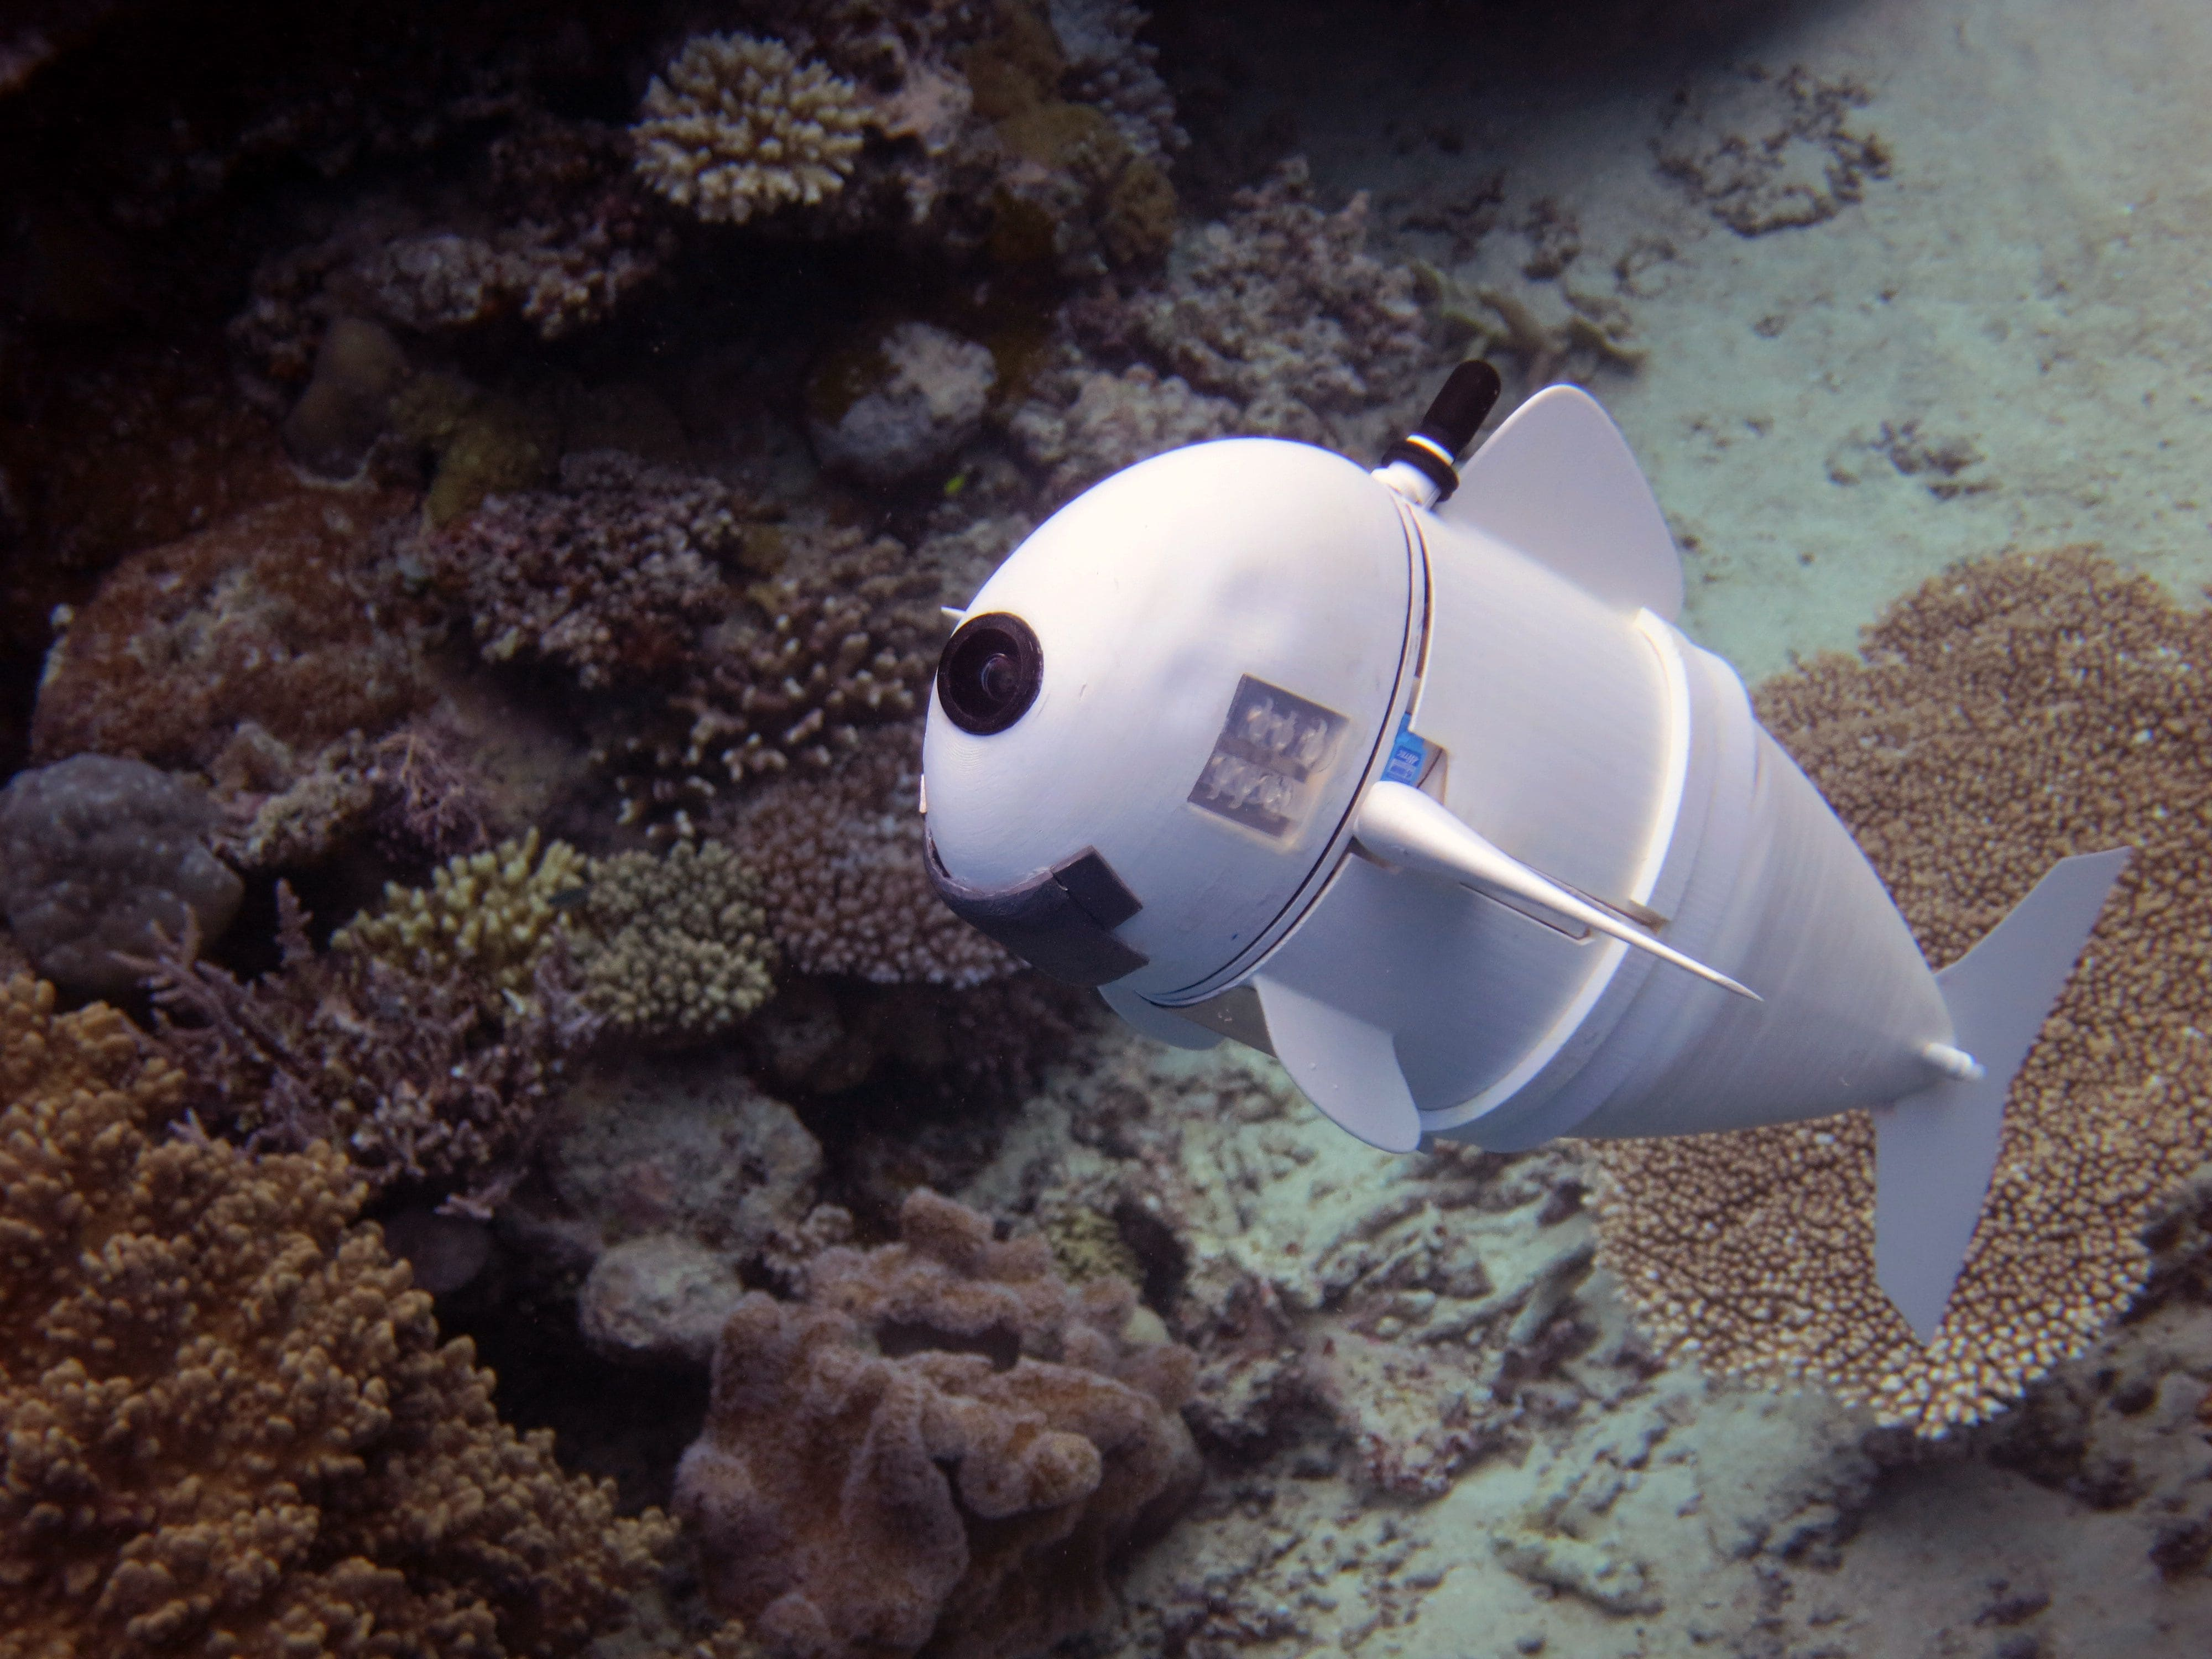
\includegraphics[width=\columnwidth]{Sofi_MIT.jpeg}%
			\caption{Le drone robotique Sofi du MIT (\href{https://www.csail.mit.edu/research/sofi-soft-robotic-fish}{Lien à la page web})}
			\label{fig:sofi-mit}
		\end{subfigure}
		\caption[]{Cas d'application pour les problèmes d'optimisation dans la WP3.}%
		\label{fig:optmisation}%
	\end{figure}
	
	
	\section{Mise en \oe{}vre du projet}
	
	\subsection{Objectifs et échéances}
	
		\begin{figure}[htb]
		\begin{center}
			\begin{ganttchart}[y unit title=0.6cm,
				y unit chart=0.6cm, 
				x unit=0.4cm,
				vgrid,hgrid, 
				title label anchor/.style={below=-1.6ex},
				title left shift=.05,
				title right shift=-.05,
				title height=1,
				progress label text={},
				bar height=0.7,
				group right shift=0,
				group top shift=.6,
				group height=.4]{1}{30}
				%labels
				\gantttitle{Dur\'ee totale}{30} \\
				\gantttitle{$T_0 + 12$}{6} 
				\gantttitle{$T_0 + 24$}{6} 
				\gantttitle{$T_0 + 36$}{6} 
				\gantttitle{$T_0 + 48$}{6} 
				\gantttitle{$T_0 + 60$}{6} \\
				%tasks
				\ganttbar{Partenariats}{1}{2} \\
				\ganttbar{Code SCRIMP}{1}{1} \\
				\ganttbar{1$^\circ$ th\`ese}{4}{21} \\
				\ganttbar{2$^\circ$ th\`ese}{10}{27} \\
				\ganttbar{3$^\circ$ th\`ese}{13}{30} \\
				\ganttbar{Post-Doc}{16}{27} \\
				\ganttmilestone{1$^\circ$ livrable}{18}\\
				\ganttmilestone{2$^\circ$ livrable}{24}\\	
				\ganttmilestone{3$^\circ$ livrable}{27}\\			\ganttbar{Soutenances}{22}{30} \\
				\ganttbar{Publications}{25}{30} 
				%relations 
				\ganttlink{elem0}{elem2} 
				\ganttlink{elem0}{elem4} 
				\ganttlink{elem1}{elem2} 
				\ganttlink{elem1}{elem3} 
				\ganttlink{elem1}{elem5}
				%\ganttlink{elem2}{elem5}
				%\ganttlink{elem3}{elem5}
				\ganttlink[link/.append style={blue,  ultra thick}]{elem2}{elem6}
				\ganttlink[link/.append style={blue,  ultra thick}]{elem3}{elem7}
				\ganttlink[link/.append style={blue,  ultra thick}]{elem4}{elem8}	
				\ganttlink[link/.append style={blue,  ultra thick}]{elem5}{elem8}		\end{ganttchart}
		\end{center}		
		\caption{Gantt Chart du projet.}
	\end{figure}
	
	Le travail sera effectué au sein du département DISC de l'ISAE. Le développement du projet se déroulera selon les objectifs et livrables suivants:
	\begin{itemize}
		\item \textbf{T0 + 6 mois} : Création des partenariats académiques et industriels.
		Pour ce qui concerne l'architecture logicielle pour le Calcul Haute Performance, on cherchera à organiser la première thèse en collaboration avec le CEA\footnote{Commissariat à l'énergie atomique et aux énergies alternatives}. Cette institution possède l'un des centres de calcul les plus sophistiqués de France. Il est donc logique d'envisager la création d'une thèse en cotutelle avec cette institution. On cherchera également à effectuer une collaboration avec Airbus pour ce qui concerne la partie optimisation.
		\item \textbf{T0 + 36 mois} : Premier livrable (\textbf{L1}) : code pour la simulation couplée pour l'interaction fluide-structure (\textbf{WP1}). Pour cette t\^ache il sera possible de reprendre le code SCRIMP développé dans le cadre de ma thèse. Le logiciel sera accompagné des tutoriaux démonstratifs.
		\item \textbf{T0 + 48 mois} : Deuxième livrable (\textbf{L2}) : création d'un code de calcul capable d'extraire des modèles réduits à partir des données des simulations haute fidélité (\textbf{WP2}). Les performances du code seront validées sur la base du trade-off gain de temps et fidélité au modèle non réduit.
		\item \textbf{T0 + 54 mois} : Troisième livrable (\textbf{L3}) : code pour l'optimisation des modèles réduits (\textbf{WP3}). La fiabilité de l'approche sera démontrée grâce à la comparaison des résultats obtenus sur les modèles haute fidélité et réduits. 
		\item \textbf{T0 + 60 mois} : Livrable final regroupant les différents codes. 		Publications et valorisation des résultats. 
	\end{itemize} 
\vspace{5pt}
Pour accomplir les objectifs, des recrutements seront effectués :
	\begin{itemize}
		\item \textbf{T0 + 6 mois} : Recrutement du premier doctorant, chargé du livrable \textbf{L1}. Le doctorant devra avoir des compétences en mathématiques appliquées et modèles pour l'ingénierie.
		\item \textbf{T0 + 18 mois} : Recrutement du deuxième doctorant, responsable du livrable \textbf{L2}, en collaboration avec Charles Poussot-Vassal de l'ONERA. Pour cette thèse, on cherchera des compétences en calcul scientifique et intelligence artificielle.
		\item \textbf{T0 + 24 mois} : Recrutement du troisième doctorant, responsable du livrable \textbf{L3}. Pour cette thèse, on cherchera un profil ingénieur avec des compétences solides en mécanique. Ce thésard travaillera avec Joseph Morlier (département DMSM de l'ISAE).
		\item \textbf{T0 + 30 mois} : Recrutement d'un chercheur post-doctoral expert en optimisation, co-responsable du livrable \textbf{L3}. La personne recruté utilisera ses compétences pour indiquer les meilleurs solutions au niveau algorithmique pour implémenter un code d'optimisation performant.
	\end{itemize}
	


	
	\subsection{Choix de l'institution d'accueil}
	Pour ce projet, on choisit l'ISAE-SUPAERO et sa grande expertise dans le domaine aéronautique. En effet les applications aéronautiques sont centrales dans ce projet. De plus, l'intégration des compétences diverses au sein de l'institution permettra le dialogue entre experts dans les différentes disciplines requises : calcul numérique et intelligence artificielle (département DISC), aérodynamique (DAEP\footnote{Département Aérodynamique et propulsion}), réduction de modèles (DCAS\footnote{Département Conception et Conduite des véhicules Aéronautiques et Spatiaux}), optimisation structurelle (DMSM).
	
	
	\subsection{Budget}

	\begin{center}
		\begin{tabular}{|c|c|}
			\hline
			D\'epense & Co\^{u}t en \euro \\
			\hline
			Porteur du projet (temps plein) & $5\times 60000=300000$ \\
			3 doctorants (temps plein) & $3\times 3\times 40000=360000$  \\
			1 Post-Doc (temps plein) & $2\times 55000=110000$ \\
			Personnels ISAE-SUPAERO & $100000$ \\
			Matériel  et calcul HPC & $70000$ \\
			Frais annexes (conférences, workshops) & $60000$ \\
			\hline
			\textbf{Total} & 1000000 \\
			\hline
		\end{tabular}
	\end{center}
	
	
	
	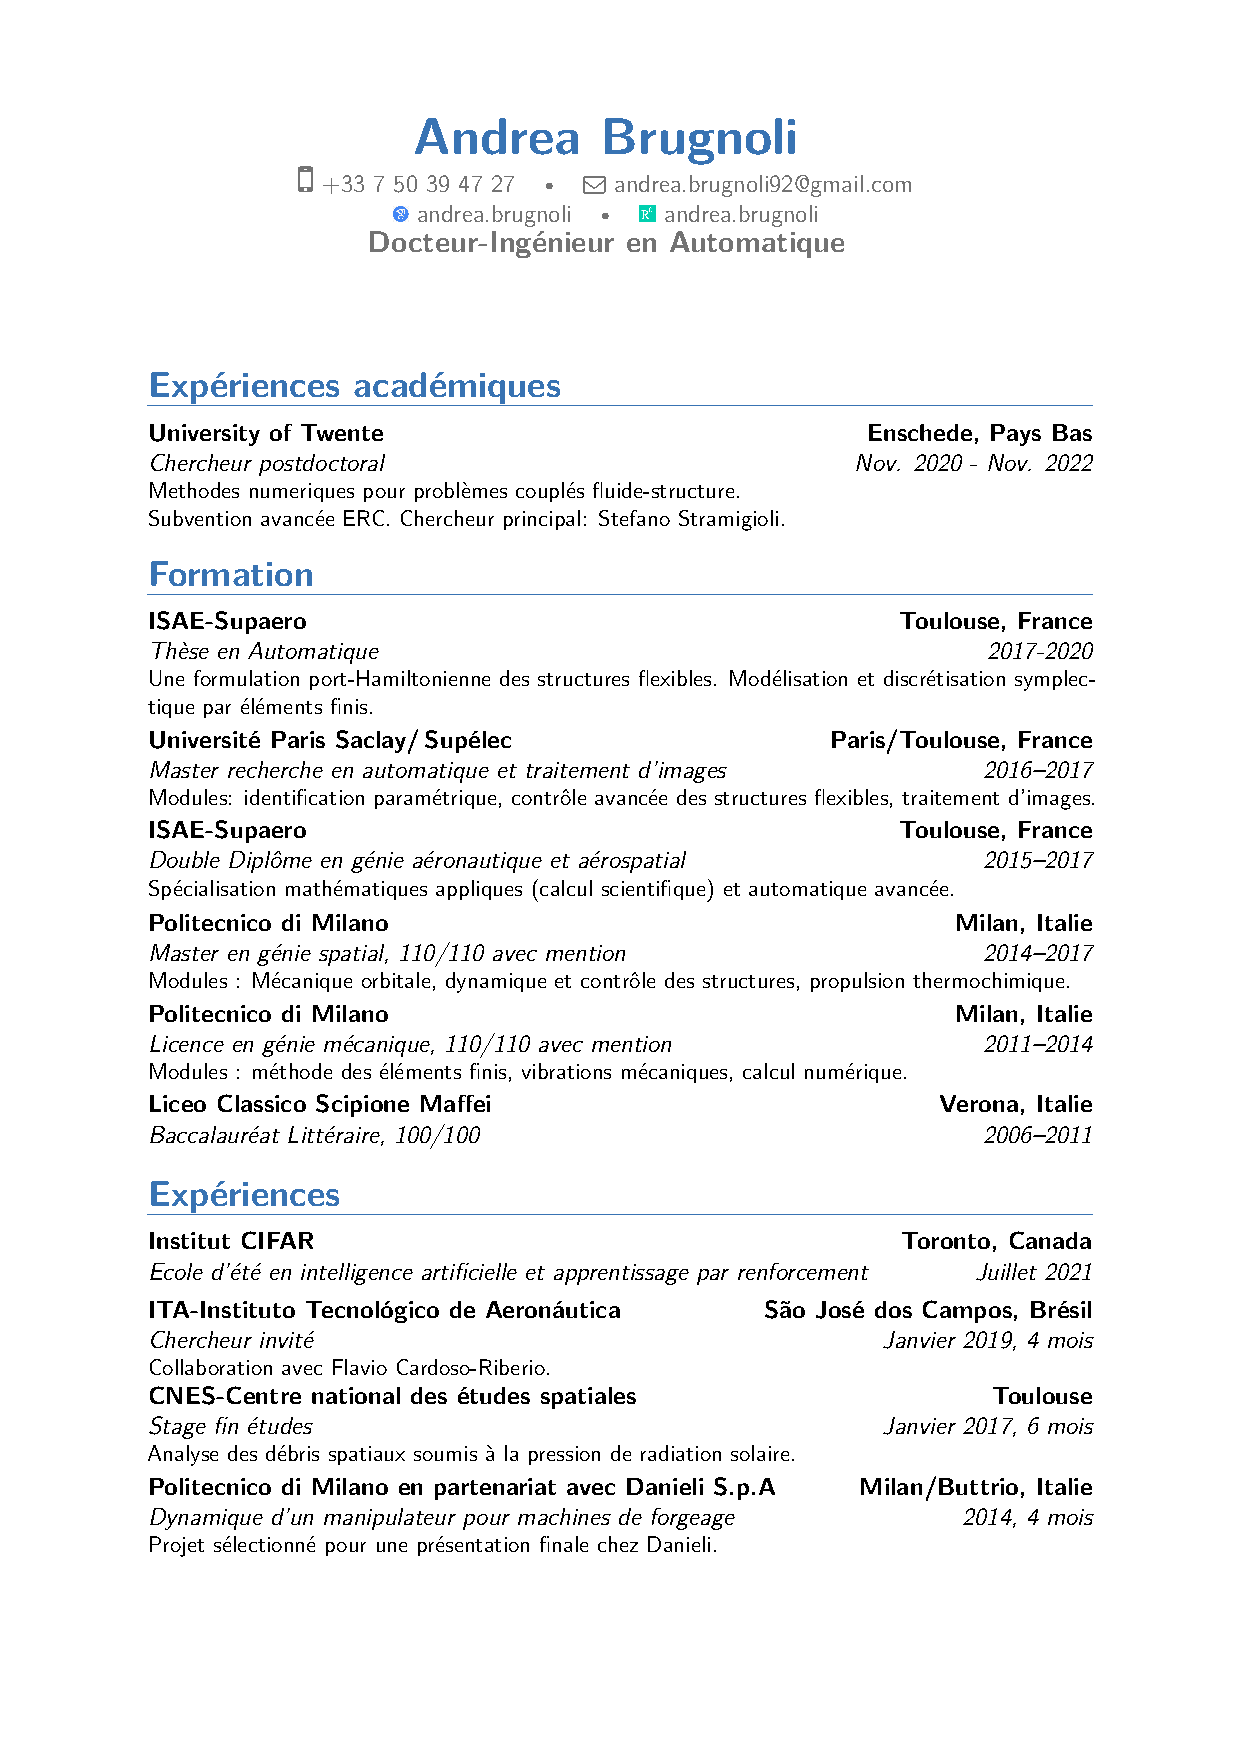
\includepdf[pages=1, pagecommand=\section{Curriculum Vitae}, offset=0 -.5cm]{cv_french.pdf}
	\includepdf[pages=2-,pagecommand={}]{cv_french.pdf}
	
	\section{Plan de carrière}
	
	La technologie, les sciences et leur impact sur l'humain m'ont toujours intéressé. C'est pour cela que j'ai effectué mes études en ingénierie dans des institutions prestigieuses (double diplôme Politecnico di Milano et ISAE-SUPAERO et master de recherche en collaboration avec Supélec/Université Paris Saclay). Mes études ont été centrées sur le calcul numérique, les systèmes dynamiques et l'automatique. Mon intérêt pour la simulation des problèmes physiques m'a amené au centre national d'études spatiales (CNES) pour mon stage de fin d'études. Dans ce stage, j'ai utilisé et développé un simulateur pour étudier le comportement des débris spatiaux sujets à la pression de radiation solaire. \\
	
	L'ISAE-SUPAERO a financé le projet de thèse pour lequel j'ai été sélectionné. Dans ce travail, j'ai exploré le potentiel d'un formalisme mathématique pour la modélisation des systèmes mécaniques complexes. J'ai pu développer des compétences à l'intersection des mathématiques appliquées, de la physique et de l'ingénierie des systèmes. La révolution digitale qui est en cours actuellement donne aux ingénieurs des instruments puissants pour pousser les avancées techniques. Je considère l'expertise acquise pendant la thèse comme fondamentale, car maintenant je possède les compétences nécessaires pour être acteur de cette révolution. Cette même expertise m'a permis d'être sélectionné comme chercheur post-doctoral dans un projet subventionné par l'European Research Council (ERC) à l'université de Twente. Ce projet est extrêmement passionnant car il réunit différents chercheurs travaillant sur les aspects théoriques et/ou pratiques de la robotique pour perfectionner le design d'un drone bio-inspiré. \\
	
	\`A moyen terme je souhaite postuler comme ingénieur de recherche ou maître de conférence dans une Université ou un Laboratoire en France. Je veux continuer à travailler dans la modélisation mathématique pour l'ingénierie, entre les mathématiques appliquées et l'informatique. Mon idéal serait de travailler dans un organisme qui cherche à résoudre des problèmes d'intérêt sociétal, en utilisant les outils de l'ingénierie computationnelle.  Si le projet MORPHEUS est sélectionné pour le prix Lopez-Loreta, je me consacrerai à plein temps à sa réalisation. Ce projet touche à différentes thématiques qui sont au centre de mes intérêts. La possibilité de pouvoir le financer pendant 5 ans représente une opportunité unique de croissance professionnelle. J'envisage également de soutenir une Habilitation à Diriger des Recherches dans un horizon de moins de 10 ans.
	
	
	\section{Production scientifique}
	{
		\nocitearticle{brugnoli2019ammmin,brugnoli2019ammkir,brugnoli2020msd,brugnoli2021ther,brugnoli2021num,califano2021,brugnoli2022df}
		\bibliographystylearticle{alpha}
		\bibliographyarticle{biblio_articles}
		
		\nociteconf{brugnoli2019cpde,brugnoli2019cdc,cardoso2019cdc,brugnoli2020wc,brugnoli2020mtns,brugnoli2021vk,cherifi2021data,rashad2021ext}
		\bibliographystyleconf{alpha}
		\bibliographyconf{biblio_conf}  
		
		\nociteconfnoproc{brugnoli2021siamcse}
		\bibliographystyleconfnoproc{alpha}
		\bibliographyconfnoproc{biblio_confnoproc}   
	}
	
	
	\section{Réussites professionnelles}
	
	Pendant mon parcours professionnel, j'ai pu vivre des moments extrêmement gratifiants. \\
	
	En premier, l'obtention de mon doctorat, défendu face à une jury d'experts internationaux, venants de France, Italie et Belgique. La qualité du travail a été reconnue à l'unanimité par les membres du jury et également par la fondation ISAE-SUPAERO, qui m'attribué un des 5 prix de thèse 2021 (la vidéo de présentation de mon travail peut être visualisée à ce lien \url{https://www.youtube.com/watch?v=2nNE4LgIkzA}). \\
	
	Les travaux effectués dans le cadre de ma thèse ont donné lieu à 5 articles dans des revues scientifiques de haut niveau \citearticle{brugnoli2019ammmin,brugnoli2019ammkir,brugnoli2020msd,brugnoli2021ther,brugnoli2021num} (\textit{Applied Mathematical Modelling}, \textit{Multibody System Dynamics}, \textit{Journal of Thermal Stresses}). La portée du travail est démontrée par le fait que ces journaux touchent à des aspects différents de la modélisation mathématique en ingénierie. Dans le cadre de ma thèse, j'ai aussi effectué une  mobilité à l'ITA, Istitito Techn\'ologico de Aeron\'autica (São José dos Campos, Brésil). Ce séjour, qui à donné lieu à trois contributions dans des conférences internationales prestigieuses \citeconf{brugnoli2019cdc,cardoso2019cdc,brugnoli2020wc}, m'a énormément enrichi au niveau professionnel et humain; en particulier j'ai pu découvrir les activités de recherche entre l'ITA et la compagnie aérienne Embraer, centrées sur la caractérisation des non-linéarités géométriques pour des avions expérimentaux très souples.  \\
	
	La dernière expérience que je souhaite mentionner a été mon déménagement aux Pays-Bas pour travailler au sein du projet Portwings. Cet ambitieux projet demande des compétences extrêmement diversifiées et chaque membre du groupe est en effet responsable d'une thématique spécifique. Ma mission est de mettre en place les algorithmes numériques pour la simulation du vol battu des oiseaux, qui représente un exemple extrêmement compliqué d'interaction fluide-structure. J'ai pu m'intégrer rapidement, en arrivant à instaurer une discussion scientifique très constructive avec des chercheurs ayant une formation différente de la mienne. Mon travail a déjà donné lieu à un article de revue soumis à un journal très réputé dans le domaine de la physique computationelle \citearticle{brugnoli2022df}. 
	
	
	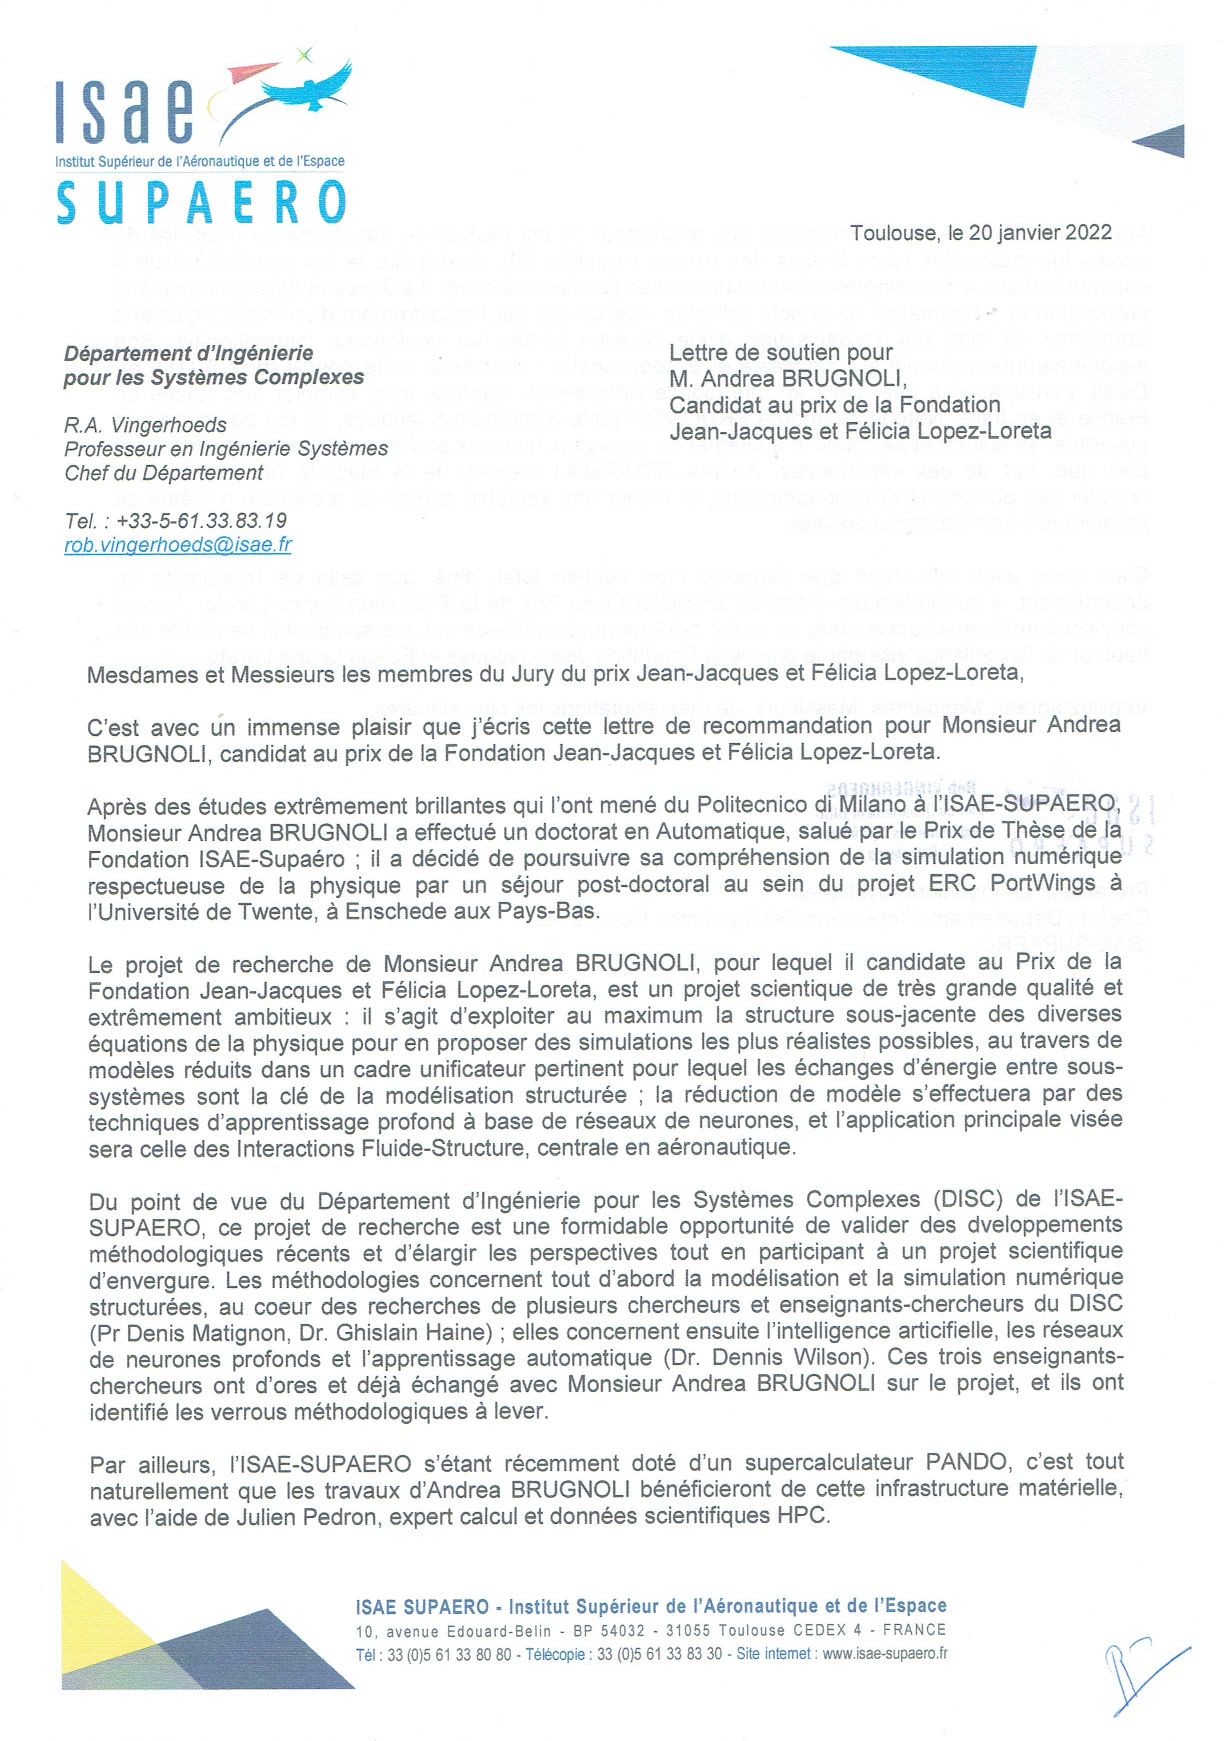
\includepdf[pages=1, pagecommand=\section{Lettre d'invitation de l'institution d'accueil}]{./Letters/gsLettreDISC.pdf}
	\includepdf[pages=2-,pagecommand={}]{./Letters/gsLettreDISC.pdf}
	
	\section{Description de l'institution d'accueil}
	
	L'ISAE-SUPAERO est un établissement public à caractère scientifique, culturel et professionnel (EPSCP) sous tutelle de la DGA du ministère des armées. Implanté à Toulouse, il est une référence mondiale de la formation et de la recherche dans les domaines aéronautiques, spatial et systèmes connexes. L'Institut délivre des
	formations de haut niveau d'ingénieurs, de masters, de masters spécialisés et de doctorats aux débouchés diversifiés. L'ISAE-SUPAERO mène également des activités de recherche et développement et dispose de 6 départements:
	\begin{itemize}
		\item Aérodynamique, énergétique et propulsion (DAEP);
		\item Conception et conduite des véhicules aérospatiaux (DCAS);
		\item Mécanique des Structures et Matériaux (DMSM);
		\item Ingénierie des Systèmes Complexes (DISC); 
		\item Électronique, Optronique et traitement du Signal (DEOS);
		\item Langues Arts Culture et Société (LACS).
	\end{itemize}

	\appendix
	
	\section{Lettres de manifestations d'intérêt}
	
	\`A support du fait que le projet MORHPEUS présente un fort intérêt industriel et académique, j'ai engagé des discussions avec des acteurs industriels dans le domaine aérospatial, ainsi que avec des centres de recherche très réputés pour leur compétences en simulation numérique et intelligence artificielle, et des professeurs universitaires. 
	
	Les personnes suivantes ont donné leur support au projet:
	\begin{itemize}
		\item Isabelle Bloy, Head of Single aisle  à Airbus et responsable du programme A321 XLR dans le département New developments in Chief Engineering.
		\item Michele Colombo, Technical Specialist Digital Enablers à Airbus, est spécialiste technique pour la partie Intelligence Artificielle et aéroélasticité.
		\item Catherine Lambert, présidente du Cerfacs\footnote{Centre Européen de Recherche et Formation Avancée en Calcul Scientifique}, est une experte en traitement du signal et compression de données. 
		\item Corentin Lapeyre, coordinateur principal de l'equipe Helios au Cerfacs, est un expert dans le domaine de l'IA appliquée à la physique computationnelle.
		\item Pierre-Henri Maire, Directeur de la Recherche au CEA à Bordeaux, est un expert dans le domaine de la physique computationnelle.
		\item Volker Mehrmann, Président de l'association européenne des mathématiques et professeur à TU Berlin, est un mathématicien spécialisé dans le développement d'algorithme numériques pour les applications industrielles (réduction de modèle et contrôle optimal).
		\item Stefano Stramigioli, Vice Président of euRobotics et professeur à l'Université de Twente, est un roboticien spécialisé dans les systèmes port-Hamiltoniens et leur utilisation pour le contrôle de manipulateurs robotiques.
	\end{itemize}

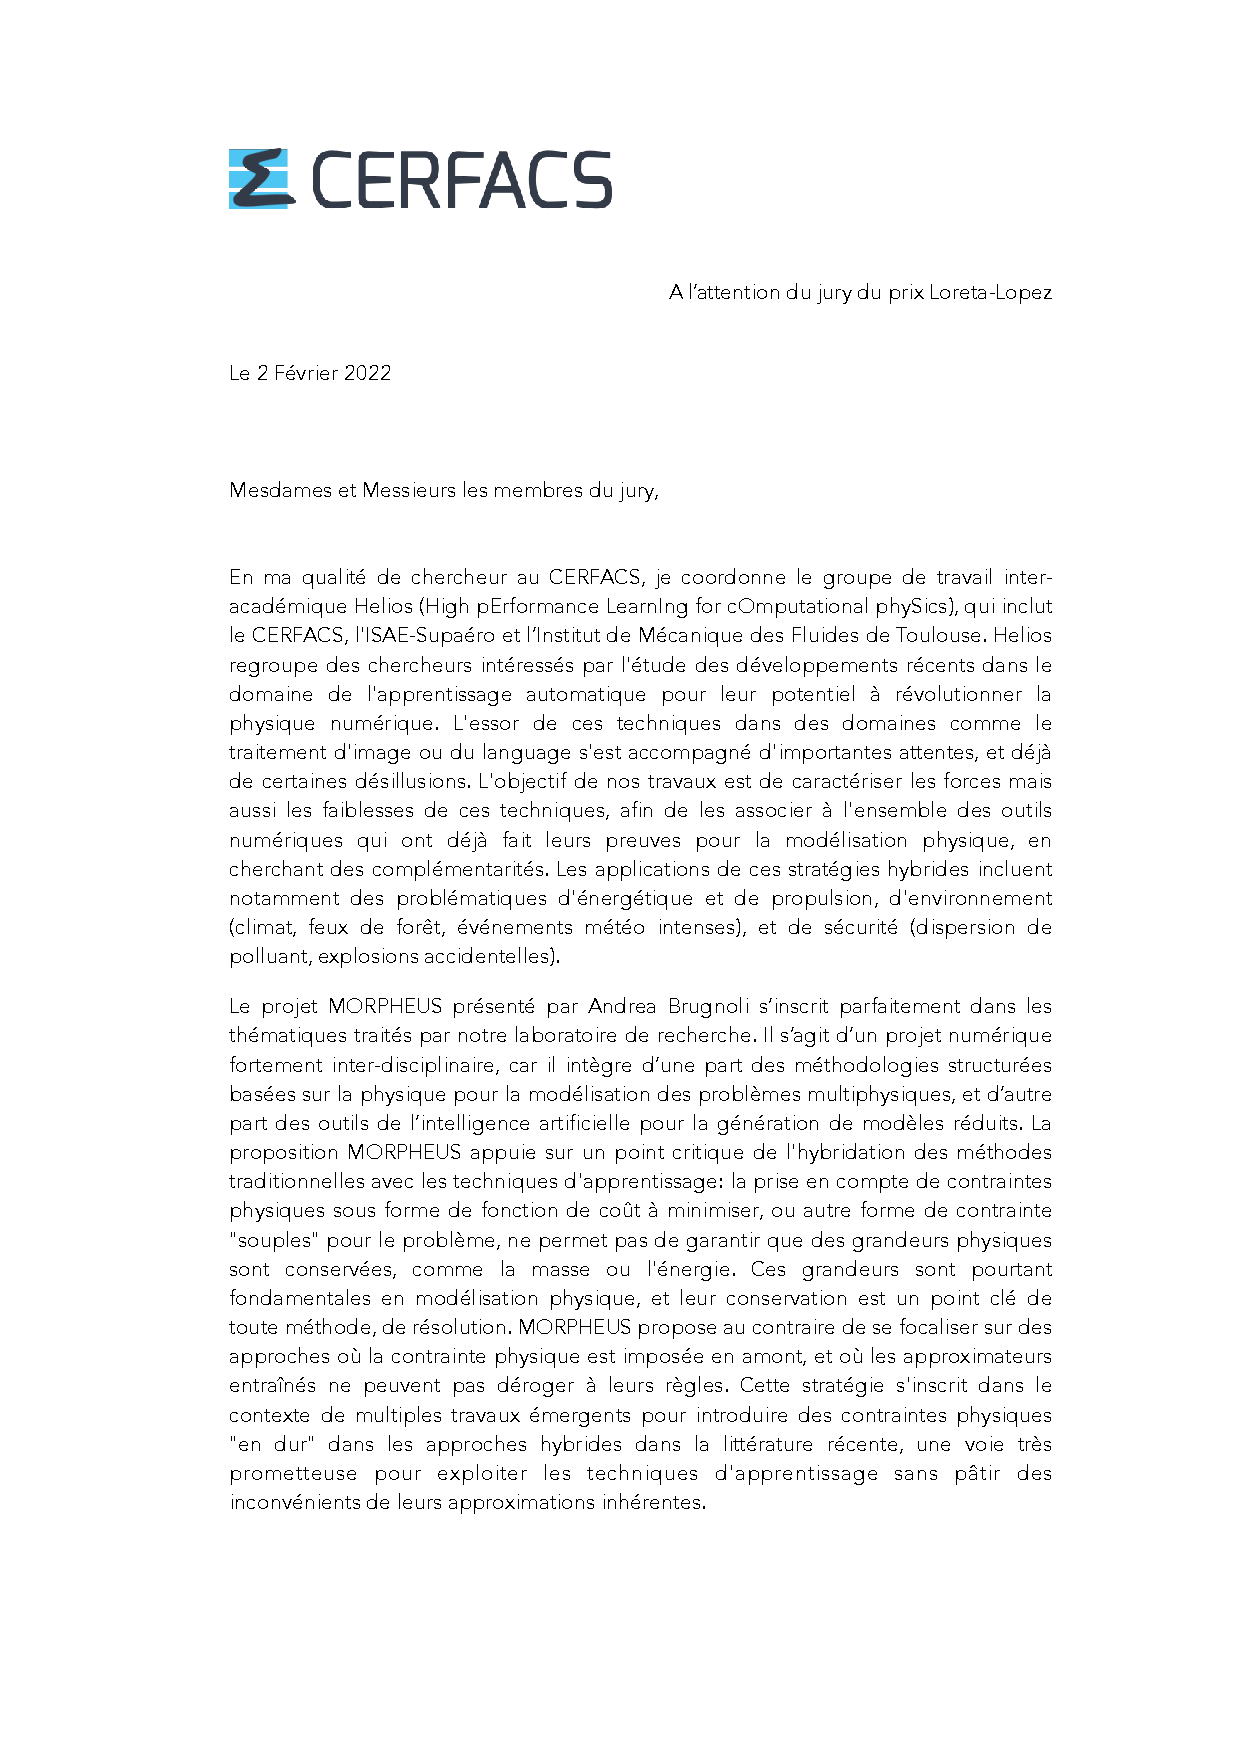
\includepdf[pages=1-]{./Letters/Lettre_Soutien_Lapeyre.pdf}


\section{Les systèmes port-Hamiltoniens}\label{sec:pHreview}

Dans cette annexe la théorie des systèmes port-Hamiltoniens est rapidement présentée. La discussion reprends l'introduction du livre \cite{van2014port}. \\

La théorie des systèmes port-Hamiltoniens rassemble différentes traditions dans la modélisation et l'analyse des systèmes physiques. Premièrement, du point de vue de la modélisation, elle trouve son origine dans la modélisation basée sur les ports, lancée par Henry Paynter à la fin des années 50. Ce formalisme vise à fournir un cadre unifié pour la modélisation de systèmes appartenant à différents domaines physiques (mécanique, électrique, hydraulique, thermique, etc.). Ceci est réalisé en reconnaissant l'énergie comme \textit{lingua franca} entre les domaines physiques, et en identifiant des composants idéaux capturant les principales caractéristiques physiques (stockage d'énergie, dissipation d'énergie, routage d'énergie, etc.).  \\

Une deuxième origine de la théorie des systèmes port-Hamiltoniens est la mécanique géométrique. Dans ce branche de la physique mathématique la formulation Hamiltonienne de la mécanique classique est formalisée de manière géométrique. Le paradigme de base
de la mécanique géométrique consiste à représenter la dynamique Hamiltonienne d'une manière intrinsèque, c'est à dire sans introduire des coordonnées, en utilisant un espace d'état doté d'une structure symplectique ou de Poisson, ainsi que d'une fonction Hamiltonienne représentant l'énergie. Cette
approche géométrique a conduit à une théorie élégante et puissante pour
l'analyse du comportement dynamique des systèmes Hamiltoniens, affichant leurs caractéristiques, telles que les symétries et quantités conservées, de manière transparente. \\

\begin{figure}{hbt}
	\begin{center}
		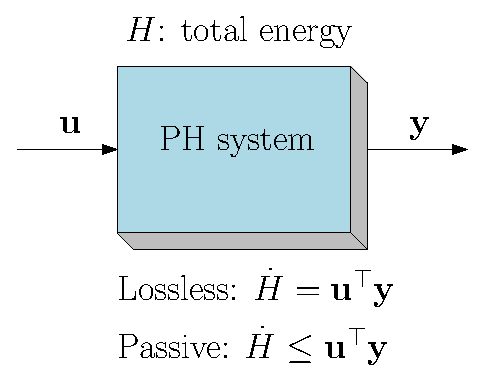
\includegraphics[width=0.35\textwidth]{sketch_PH.eps}
	\end{center}
	\caption{Un système port-Hamiltonien est un système Hamiltonien sujet \`a l'interaction avec le monde extérieur.}
	\label{fig:sketchPH}
\end{figure}

Enfin, un troisième pilier sous-jacent au cadre des systèmes port Hamiltoniens est la théorie des systèmes et du contrôle, o\'u les systèmes dynamiques sont décrits comme étant ouverts à l'interaction avec l'environnement (par exemple via des entrées et des sorties, cf. Fig. \ref{fig:sketchPH}) et comme étant susceptibles d'être contrôlées activement. \\


Une différence principale entre la théorie des systèmes port-Hamiltoniens et la mécanique géométrique réside dans le fait que pour la première la structure géométrique sous-jacente n'est pas nécessairement la structure symplectique de l'espace des phases, mais est en fait déterminée par la structure d'interconnexion du système.  En ce sens la théorie port-Hamiltonien fusionne intrinsèquement la géométrie avec la théorie des réseaux, grace \`a la notion de structure de Dirac. Une propriété clé des structures de Dirac est le fait que leur composition est à nouveau une structure de Dirac. Cela a pour conséquence cruciale que l'interconnexion des systèmes port-Hamiltoniens par leur ports est à nouveau un système port-Hamiltonien (cf. Fig. \ref{fig:intPH}). Une autre extension de la théorie des systèmes port-Hamiltoniens par rapport à la mécanique géométrique est l'inclusion d'éléments dissipateurs d'énergie, qui sont largement absents dans les systèmes Hamiltoniens classiques. Cette inclusion élargit considérablement le domaine d'application des systèmes port-Hamiltoniens par rapport à celui des systèmes Hamiltoniens classiques. \\

La modélisation port-Hamiltonien apparaît comme une théorie générale pour la modélisation des systèmes physiques complexes rencontrés dans de nombreux domaines de l'ingénierie.


	\begin{figure}[b]
	\begin{subfigure}[t]{0.45\textwidth}
		\includegraphics[width=\columnwidth]{sketch_PH_gyrator.eps} 
		\caption{Gyrateur}
		\label{fig:pHsys_gyr}
	\end{subfigure}\hfill
	\begin{subfigure}[t]{0.45\textwidth}
		\includegraphics[width=\columnwidth]{sketch_PH_transformer.eps}%
		\caption{Transformer}
		\label{fig:pHsys_tran}
	\end{subfigure}
	\caption[]{Interconnexion des deux systèmes port-Hamiltonien: ces deux type d'interconnexion sont telles \`a préserver les échanges de puissance entre les deux systèmes.}%
	\label{fig:intPH}%
\end{figure}


\section{Le code SCRIMP}\label{sec:SCRIMP}
Le code SCRIMP (Simulation and ContRol of Interactions in Multi-Physics) est un projet Python pour l'approximation numérique d'équations aux dérivées partielles contrôlées \`a la frontière en utilisant le formalisme port-Hamiltonien. La principale motivation derrière le développement de SCRIMP était de fournir un cadre facile à utiliser pour la solution numérique des systèmes port-Hamiltoniens de dimension infinie à des fins à la fois de recherche et d'enseignement. Les approximations numériques avec des discrétisations sont gérées par le logiciel d'éléments finis FEniCS (\url{https://fenicsproject.org/}). Des applications basés sur des équations aux dérivées partielles paraboliques ou hyperboliques sont abordées. Plusieurs cahiers sont fournis pour démontrer l'utilisation de SCRIMP dans ce cadre \url{https://zenodo.org/record/4945329\#.YflFPVvMJH5}.
	
\bibliographystyle{unsrt}
\bibliography{biblio_dossierLL}
	
	
\end{document}
